% !TEX program = xelatex
% 공통수학2 · Ⅰ. 도형의 방정식 · 03 점과 직선 사이의 거리 · 1/2차시
% 학생용 활동지 (답안 없음)

\documentclass[11pt,a4paper]{article}

\usepackage{kotex}
\usepackage{iftex}
\ifPDFTeX\else
  \setmainhangulfont{Noto Serif CJK KR}
  \setsanshangulfont{Noto Sans CJK KR}
\fi

\usepackage[margin=2.1cm]{geometry}
\usepackage{parskip}
\usepackage{enumitem}
\usepackage{array}
\usepackage{tabularx}
\usepackage{xcolor}
\usepackage{amssymb}
\usepackage{tikz}
\usepackage[most]{tcolorbox}
\usepackage{fancyhdr}
\usepackage{titlesec}

\definecolor{goldc}{HTML}{B07C22}
\definecolor{goldstrong}{HTML}{8A5F16}
\definecolor{indigoc}{HTML}{2B3B57}
\definecolor{indigosoft}{HTML}{6E82A6}
\definecolor{linec}{HTML}{D6DACB}
\definecolor{surface2}{HTML}{E4E8DC}
\definecolor{writeline}{HTML}{C7CCBA}
\definecolor{inksoft}{HTML}{52604F}

\titleformat{\section}{\normalfont\sffamily\bfseries\large\color{indigoc}}{\thesection}{0.6em}{}
\titlespacing{\section}{0pt}{14pt}{6pt}

\newtcolorbox{goalbox}{enhanced, breakable, colback=white, colframe=goldc, boxrule=0.5pt, leftrule=3pt, arc=2pt, left=10pt, right=10pt, top=8pt, bottom=8pt}
\newtcolorbox{sheetbox}{enhanced, breakable, colback=white, colframe=linec, boxrule=0.6pt, arc=3pt, left=11pt, right=11pt, top=9pt, bottom=9pt}

\newcommand{\writespace}[1]{%
  \par\nobreak\vspace{3pt}
  \foreach \n in {1,...,#1} {%
    \noindent\textcolor{writeline}{\rule{\linewidth}{0.4pt}}\par\vspace{0.62cm}%
  }
}
\newcommand{\fillblank}[1]{\makebox[#1]{\hrulefill}}

\pagestyle{fancy}
\fancyhf{}
\renewcommand{\headrulewidth}{0pt}
\fancyfoot[L]{\footnotesize\color{inksoft} 공통수학2 · 2026학년도 2학기 · 지평선고등학교}
\fancyfoot[R]{\footnotesize\color{inksoft} 다음 시간 --- 03 점과 직선 사이의 거리(2)}

\begin{document}

\noindent
\begin{minipage}[b]{0.62\linewidth}
  {\sffamily\footnotesize\color{indigosoft} 공통수학2 · Ⅰ. 도형의 방정식}\\[2pt]
  {\sffamily\bfseries\Large 03 점과 직선 사이의 거리 \textperiodcentered\ 6차시}
\end{minipage}\hfill
\begin{minipage}[b]{0.36\linewidth}
  \raggedleft\small\color{inksoft}
  반\ \fillblank{1.6cm} \quad 번호\ \fillblank{1.6cm}\\[4pt]
  이름\ \fillblank{3.6cm}
\end{minipage}

\vspace{4pt}
\noindent{\color{goldc}\rule{\linewidth}{2.2pt}}
\vspace{10pt}

\begin{goalbox}
\textbf{오늘의 목표}\\
점과 직선 사이의 거리가 수선의 길이임을 알고, 그 거리를 구하는 공식을 유도하여 활용할 수 있다.
\vspace{4pt}

\small\color{inksoft}
$\square$ 자신 있음 \quad $\square$ 조금 헷갈림 \quad $\square$ 처음 봄 \hfill (수업 전 나의 상태에 표시)
\end{goalbox}

\section{생각 열기 --- 가장 짧은 길은?}

\begin{sheetbox}
아래 그림처럼 점 P에서 직선 $l$ 위의 여러 점까지 선분을 그었다.

\begin{center}
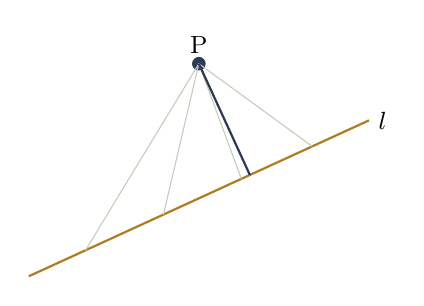
\begin{tikzpicture}[scale=0.9]
  \draw[thick, goldc] (-2.4,-0.6) -- (2.4,1.6);
  \node[right, font=\small] at (2.4,1.6) {$l$};
  \filldraw[indigoc] (0,2.4) circle (2.5pt);
  \node[above, font=\small] at (0,2.4) {P};
  \foreach \t in {-1.6,-0.5,0.6,1.6} {
    \draw[writeline, thin] (0,2.4) -- (\t, {(\t+2.4)*0.4583-0.6});
  }
  \draw[indigoc, thick] (0,2.4) -- (0.72,0.83);
\end{tikzpicture}
\end{center}

\begin{enumerate}[leftmargin=1.4em, itemsep=2pt]
  \item 여러 선분 중 가장 짧아 보이는 것은 어떤 선분인가? 직선 $l$과 어떤 각을 이루고 있는가?
  \item 점과 직선 사이의 거리를 어떻게 정의하면 좋을지 자신의 말로 적어 보자.
\end{enumerate}
\writespace{3}
\end{sheetbox}

\section{개념 정리 --- 점과 직선 사이의 거리 공식}

\begin{sheetbox}
점 P$(x_1,y_1)$에서 직선 $l\colon ax+by+c=0$에 내린 수선의 발을 H라 하면, 점과 직선 사이의 거리는 $\overline{\text{PH}}$이다. 직선 PH와 직선 $l$이 서로 \fillblank{2.4cm}이므로 두 직선의 기울기의 곱이 \fillblank{2cm}이라는 조건을 이용하면 다음 공식을 얻는다.

\[
\overline{\text{PH}} = \fillblank{6.5cm}
\]

특히, 원점과 직선 $ax+by+c=0$ 사이의 거리는
\[
\fillblank{4.5cm}
\]

\vspace{6pt}
\textbf{보기} --- 점 $(3,5)$와 직선 $4x-3y-12=0$ 사이의 거리:
\[
\dfrac{|4\cdot 3 - 3\cdot 5 - 12|}{\sqrt{4^2+(-3)^2}} = \dfrac{\fillblank{1.6cm}}{\fillblank{1.6cm}} = \fillblank{1.6cm}
\]
\end{sheetbox}

\section{연습 문제}

\begin{sheetbox}
\textbf{1.} 다음 점과 직선 사이의 거리를 구하시오.\\
\hspace*{1.6em}⑴ 점 $(2,2)$와 직선 $6x+8y-3=0$ \qquad ⑵ 원점과 직선 $y=3x-10$
\writespace{4}
\end{sheetbox}

\section{사고의 가시화 --- See · Think · Wonder}

\noindent{\footnotesize\color{inksoft} 오늘 배운 `점과 직선 사이의 거리'를 떠올리며 아래 세 칸을 채워 보자.}\\[6pt]
\begin{tabularx}{\linewidth}{@{}XXX@{}}
\textbf{\footnotesize\color{indigoc} See --- 무엇을 보았나?} &
\textbf{\footnotesize\color{indigoc} Think --- 무엇을 생각했나?} &
\textbf{\footnotesize\color{indigoc} Wonder --- 무엇이 궁금한가?} \\[4pt]
\end{tabularx}
\noindent
\begin{minipage}[t]{0.32\linewidth}\writespace{3}\end{minipage}\hfill
\begin{minipage}[t]{0.32\linewidth}\writespace{3}\end{minipage}\hfill
\begin{minipage}[t]{0.32\linewidth}\writespace{3}\end{minipage}

\section{마무리 성찰}

\begin{sheetbox}
\begin{minipage}[t]{0.48\linewidth}
{\footnotesize\color{inksoft} 오늘 배운 것을 한 문장으로}
\writespace{2}
\end{minipage}\hfill
\begin{minipage}[t]{0.48\linewidth}
{\footnotesize\color{inksoft} 감사 일기 / 유념 한 줄}
\writespace{2}
\end{minipage}
\end{sheetbox}

\end{document}
